
\begin{chapterIntro}
This chapter discusses some use-cases for middleware to handle earth system data.
\Cref{sec:use cases/climate and weather} starts with a high-level perspective to current workloads in climate and weather forecasts.
It follows an introduction of involved stakeholders/actors (see \Cref{sec:use cases/actors}) and systems (see \Cref{sec:use cases/systems}).
\Cref{sec:use cases/use cases} and following are the actual use cases.
Use cases can extend each other, and are generally constructed in a way that they are not limited to the ESDM but also apply to similar middleware.
In addition, the use of backends is kept abstract where possible, so that in principle implementations can be swapped with only minor semantic changes to the sequence of events.
\end{chapterIntro}



%%%%%%%%%%%%%%%%%%%%%%%%%%%%%%%%%%%%%%%%%%%%%%%
\section{Climate and Weather Workloads}
\label{sec:use cases/climate and weather}

The climate and weather forecast communities have their characteristic workflows and objectives, but also share a variety of methods and tools (e.g., the ICON model is used and developed together by climate and weather scientists).
This section briefly collects and groups the data-related high-level use-cases by the community and the motivation for them.

Numerical weather prediction focuses on the production of a short-time forecast based on primary sensor (satellite) data and generates derived data products for specific end users (e.g., the weather forecast for the general public or military).
As computer capabilities and requirements for users increase, new services are added, or existing services are adapted.
Climate predictions run for long periods and may involve complex workflows to compute derived information such as monthly mean or to identify specific patterns in the forecast data such as tsunamis.
%before the community settles for large scale ensemble simulations the models go two a continues process of model and performance optimisations.

In the following, a list of specific high-level workloads and use-cases that are typically performed per community is given.
These use-cases resemble what a user/scientist usually has in mind when dealing with numerical weather prediction (NWP) and climate simulation; there are several supportive use-cases from the perspective of the data centre that will be discussed later.


\paragraph{Numerical Weather Prediction}

\begin{itemize}
	\item Data ingestion: Store incoming stream of observations from satellites, radar, weather stations and ships.
	\item Pre-Processing: Cleans, adjusts observation data and then transforms it into the data format used as an initial condition for the prediction. For example, insufficient sampling makes pre-processing necessary so models can be initialised correctly.
	\item Now Casting (0-6h): Precise prediction of the weather shortly.
	Uses satellite data and data from weather stations, extrapolates radar echos.
	\item Numeric Model Forecasts (0-10+ Days): Run a numerical model to predict the weather for the next few days.
	Typically, multiple models (ensembles) are run with some perturbed input data.
	The model usually proceeds as follows: 1) Read-Phase to initialise simulation; 2) create periodic snapshots (write) for the model time, e.g., every hour.
	\item  Post Processing: create data products that may be used for multiple purposes.
	\begin{itemize}
		\item for Now Casting: multi-sensor integration, classification, ensembles, impact models
		\item for Numeric Model Forecasts: statistical interpretation of ensembles, model-combination
		\item generation of data products like GRIB files as service for customers of weather forecast data
	\end{itemize}
	\item Visualisations: Create fancy presentations of the future weather; this is usually part of the post-processing.
\end{itemize}


\paragraph{Climate}

Many use cases in climate are very similar:

\begin{itemize}
	\item Pre-processing: Similar to the NWP use case.
	\item Forecasting with Climate Models: Similar to the NWP use case, with the following differences:
	\begin{itemize}
		\item The periodic snapshots (write) uses variable depending frequencies, e.g., some variables are written out with higher frequencies than others
	\end{itemize}
	\item Post-processing: create useful data products, e.g., run CDOs (Climate Data Operations) to generate averages for certain regions. The performed post-processing depends on the task the scientist has in mind. While at runtime of the model some products are clear and may be used to diagnose the simulation run itself, later scientists might be interested in running additional post-processing to look for new phenomena.
	\item Dynamic visualisation: use interactive tools to search for interesting patterns. Tools such as VTK and ParaView are used. %Potentially create a time series movie.
	\item Archive data: The model results are stored on a long-term archive. They may be used for later analysis --  often at other sites and by another user, e.g., to search for some interesting pattern, or to serve as input data for localised higher-resolution models. Also, it supports the reproducibility of research.
\end{itemize}

Note that compared to NWP there is more dynamic and flexibility needed in climate forecasting.
Scientists may run prototypical code simulating novel features and creating new data products.
They may use many different tools on different sites to post-process and visualise data and, over time, new methods may be found to interact with data model output.

%%%%%%%%%%%%%%%%%%%%%%%%%%%%%%%%%%%%%%%%%%%%%%%
\section{Roles and Human Actors}
\label{sec:use cases/actors}

This section introduces the involved actors and provides an overview of the use cases addressed in this chapter.
Research is often funded in relatively short term projects with a set of defined improvements to state of the art.
Projects are often embedded with already existing institutions such as universities or research laboratories.
\Cref{fig:esiwace_usecases} visualises the project perspective to data creation and analysis.
An experimenter usually prepares and runs a model. The preparation may include ingestion of data (migration of data into ESD) and pre-processing this data.
An analyst analyses model output and generates useful data products.
In this process, he/she may retrieve a selected subset of data to a local machine to foster rapid data exploration.
These use cases shall be supported on an exascale demonstrator.
In general, we refer to scientists as users of ESDM.



\begin{figure}
	\centering
	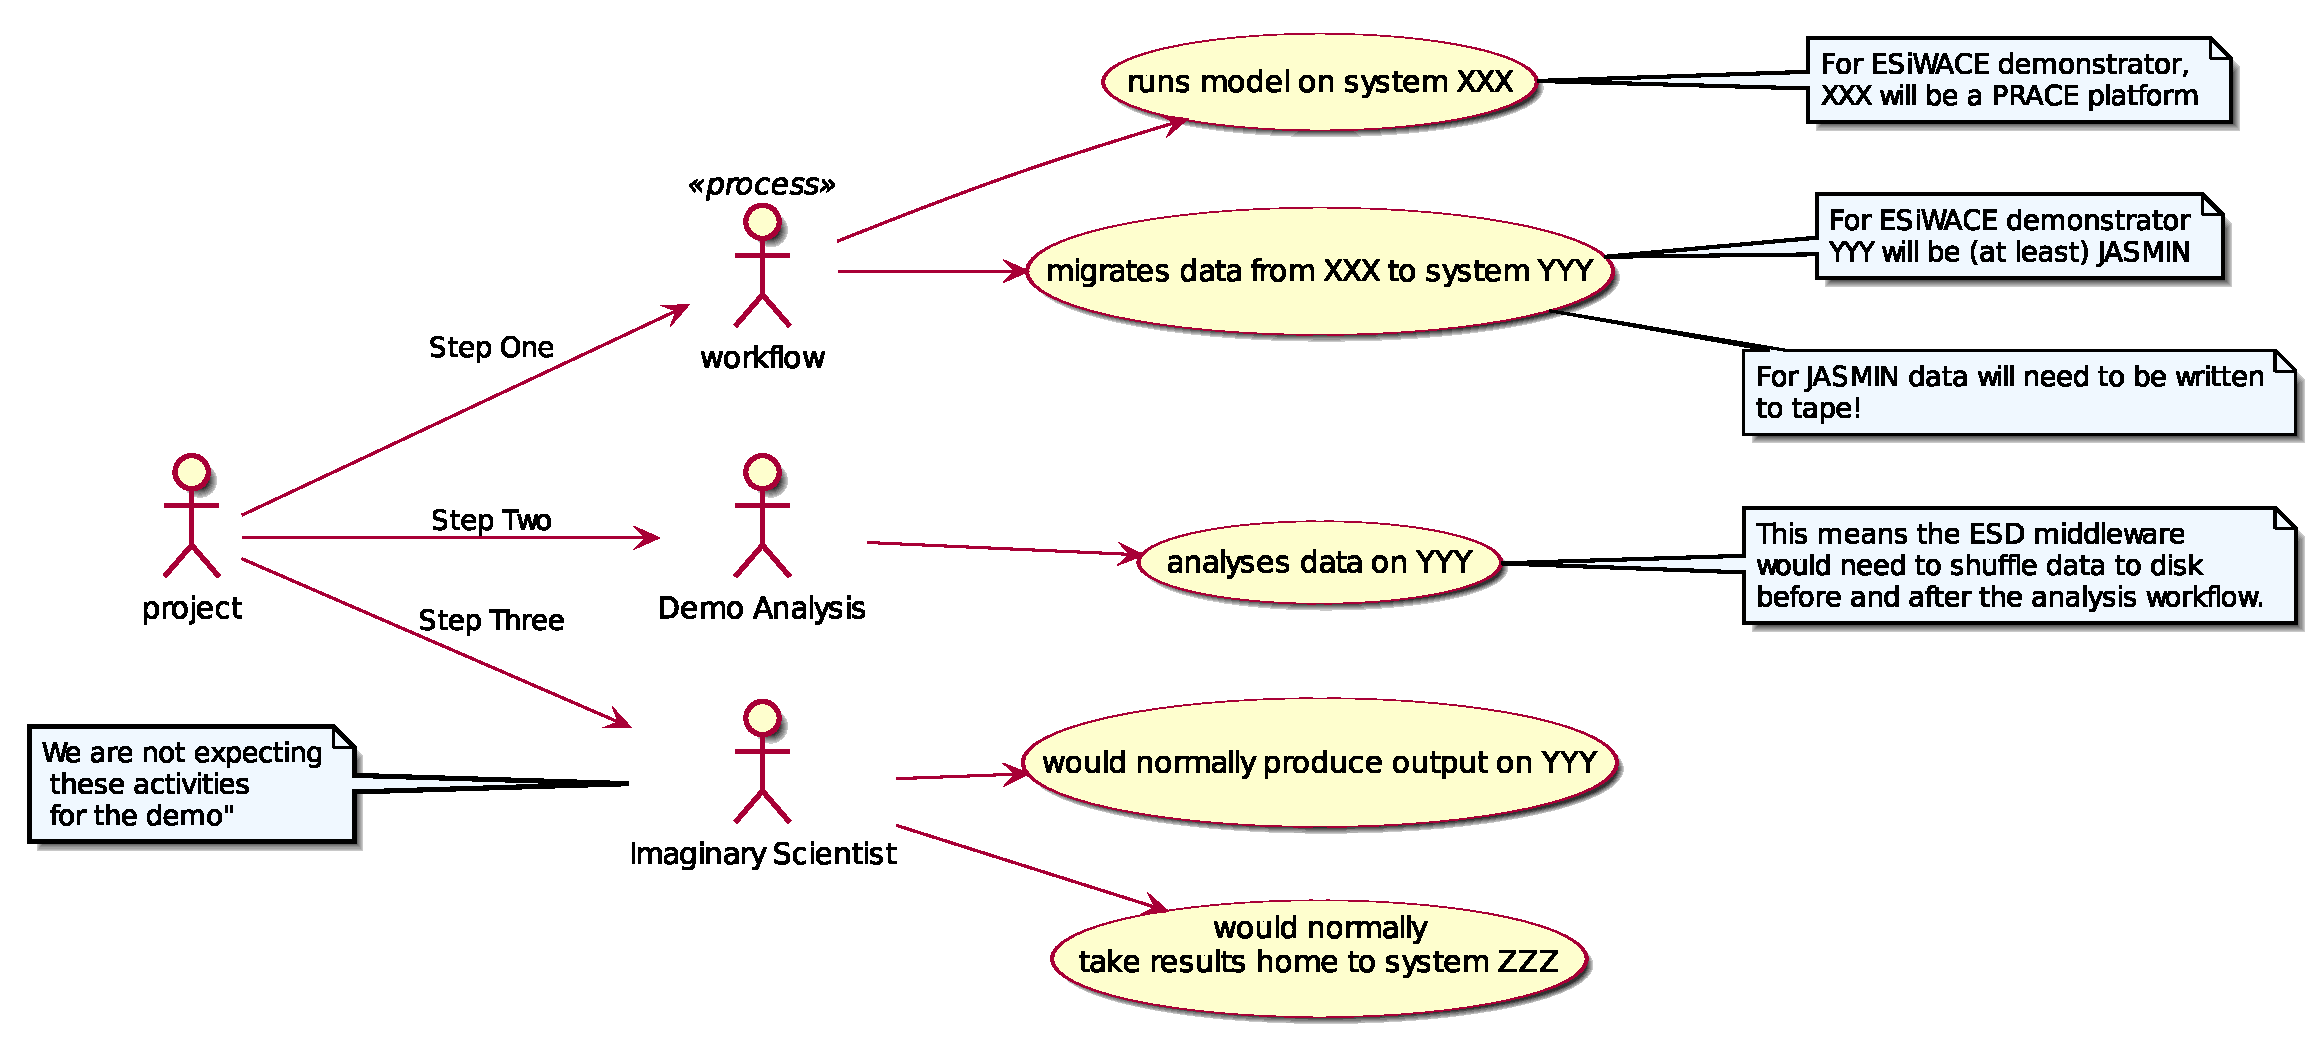
\includegraphics[width=0.75\linewidth]{use-cases/uml/generic/esiwace_usecases.eps}
	\caption{Different roles and tasks commonly seen within an earth system related project.}
	\label{fig:esiwace_usecases}
\end{figure}



\medskip

Commonly, scientists share technical infrastructure such as computer and storage systems with other groups within an organisation.
But as scientists collaborate across the boundaries of their institution, the operation of, e.g., a data centre is outsourced and embedded into a separate organisation (such as the DKRZ, ECMWF or Met office) with the different organisations as stakeholders.
However, it is not uncommon to find smaller systems operated by individual research groups for analysis tasks.
%\Cref{fig:use_case_relationships} illustrates the various actors that are involved in data management within and across sites.
A role in this context does not translate to persons, but a person may fill multiple roles, but also multiple persons may collaborate on a single role.



%\begin{figure}
%	\centering
%	\includegraphics[width=0.5\linewidth]{use-cases/uml/generic/data-center-roles.eps}
%	\caption{User and data management actors in a scientific computing environment. In many cases multiple roles maybe fulfilled by the same person.}
%	\label{fig:use_case_relationships}
%\end{figure}

\medskip

The use cases described in this chapter, are illustrated in \Cref{fig:overview-actors-use-cases}.
In general, by use case we mean a typical workflow that may consist of multiple steps that are run sequentially or in parallel (concurrently).
It covers the execution of applications (Simulation),
the pre/post processing of data needed to drive applications,
the concurrent simulation and post-processing, i.e., while the simulation runs, we already produce relevant data products,
the simulation coupled with in-situ post-processing,
the simulation coupled with interactive visualisation,
the simulation coupled with tools for big data analytics.
These use cases are built on the general use cases for independent write and read.


An experimenter (user) has a use case in mind that consists of multiple steps (jobs) that are run sequentially or concurrently.
He/she submits a job of the workflow to the job scheduler which assigns resources on the supercomputer and starts the execution of the job script.
Optionally, it may use the ESDM interfaces to steer data migration and staging or further optimisations.
The job script runs on one of the allocated nodes and processes a sequence of instructions such as running of applications.
An application may use the ESDM interface directly or via an existing API such as NetCDF indirectly.




\begin{figure}
	\centering
	\includegraphics[width=\linewidth]{use-cases/uml/generic/use-case-overview-manual}
	\caption{Overview of described actors and use cases.}
	\label{fig:overview-actors-use-cases}
\end{figure}





\subsection{Credentials and Permissions of Actors for Data Access}

The introduction captured the logical view of the different actors managing and using data.
A more technical perspective can be described as follows.
Three general types of actors can interact with an earth system storage resource:

\begin{itemize}
	\item Unprivileged Users (e.g., external partners, that only download or read available data)
	\item Privileged Users (Project participants, with varying privileges)
	\item Administrators (Site/Infrastructure operators)
\end{itemize}

In the following, we use the term object to refer primarily to something with equivalent semantics to a file.
More fine-grained object access will also be available via any APIs exposed by the service.

\subsection*{Unprivileged User}

An unprivileged user is someone who has only read-only access. These users can:
\begin{itemize}
	\item navigate content, using faceted browse against public tags,
	\item list all (public) tags to which they have access,
	\item given a tag, list all tags carried by objects with the first tag,
	\item given a list of tags, list all tags carried by objects with all members of that list,
	\item given a tag list, list all objects with the union set of all those tags,
	\item retrieve any visible object from the list of objects presented by any tag list,
	\item interact with any visible object via limited read-only operations.
\end{itemize}

\subsection*{Privileged Users}

A privileged user is someone who has CRUD access to (their) content within the archive as well as all the abilities of an unprivileged user applied to their content. They can:
\begin{itemize}
	\item create, retrieve, update, and delete content within prescribed quotas,
	\item control access to their objects (see below),
	\item assign tags to objects,
	\item navigate both public or (own) private tags.
\end{itemize}

Controlling access:
\begin{itemize}
	\item Users can create ``group'' identifiers, and associated user identifiers with that group.
	\item They must themselves be members of any group they create.
	\item They can add/remove any other user identifiers known to them to that group.
	\item How users find the identifiers of other users is not defined here.
	\item If they use the identifier ``public'' for a group, then users in this group (who may also include the unique identifier ``anonymous''), then users in this group will have read-only access to these objects.
	\item Users can assign any group identifier of which they are a member of any object they create. In doing so, they make ``their'' objects into ``shared'' objects (except for the public group as defined above, where they are simply making the object read-only to that group).
	\item Any user with ``shared'' access has the same privileges for that object as the original owner, except that of modifying or removing the group tag.
	\begin{itemize}
		\item This means they can delete, update, and retrieve the object. Of course, deleting it will disassociate the group tag.
	\end{itemize}
	\item Users can list the groups of which they are members, and list the members of any of those groups.
\end{itemize}

Note that this usage of the group is not identical to the concept of UNIX groups, because users control their definition.

\subsection*{Administrators}

Administrators can:

\begin{itemize}
	\item  start and stop any service,
	\item  access all data held by all privileged users,
	\item  manage privileged users: create, update, delete users,
	\item  allocate quotas, i.e., define available storage space for users and groups,
	\item  retrieve usage information,
	\item  configure the layout of content in the service against available storage resources,
	\item  migrate content within the storage resources (a process that might temporarily disable user access while the migration takes place)
	\item configure any required computer, cache, and network services.
\end{itemize}


%%%%%%%%%%%%%%%%%%%%%%%%%%%%%%%%%%%%%%%%%%%%%%%
\clearpage
\section{Systems}
\label{sec:use cases/systems}


This section describes essential hardware and storage components that are used by the use cases.
Each system has a description, and if applicable a list of related subsystems.
In addition, for every subsystem risk factors and failure modes of the system are collected, which then can be easily addressed by the individual use cases.

Each system comes with a short description, an illustration briefly explaining the architecture, a list of associated risks as well as a list of related subsystems.
It follows a more detailed description of each section:

\paragraph{System Description:} A summary of the system, standard practices and relations to other systems.
\paragraph{Risks:} Typical risks and failure modes associated with the system.
\paragraph{Subsystems:} If the system is split into subsystems, this includes a list with references to each subsystem.

%%%%%%%%%%%%%%%%%%%%%%%%%%%%%%%%%%%%%%%%%%%%%%%%%%%%
\subsection{System: Supercomputer}
\label{System: Supercomputer}

\begin{figure}
	\centering
	\includegraphics[width=0.5\linewidth]{use-cases/systems/hpc_clean}
	\caption{A typical supercomputer with compute notes connected via a high performing network interconnect and a dedicated storage system.}
	\label{fig:system supercomputer}
\end{figure}


\paragraph{System Description:}
An HPC system here is assumed to be a cluster computer with 100 to 100.000 cores/nodes.
The nodes are connected via a network, often a specialised high-throughput, low-latency interconnect (e.g., Infiniband). An HPC system usually does not stand by itself but is also connected to a high-performance storage system.
\Cref{fig:system supercomputer} illustrates a commonly seen deployment of a supercomputer, though many details are ignored as the exact topology depends on the specific applications and systems deployed.
Resource allocations are commonly managed using a job scheduler that allows users to submit jobs.


\paragraph{Risks:}
\begin{itemize}
	\item Hardware failures (a growing concern in expectation of exascale)
	\item Data loss and corruption (silent)
\end{itemize}


\paragraph{Subsystems:}


\begin{itemize}
	\item Compute Nodes: The raw compute resources. CPUs + Memory
	\item Storage System: A network attached storage system. Disk/SSD based, and maybe long-term (e.g., Tape) (see \Cref{System: Storage System})
	\item Applications (see \Cref{System: Application})
	\item Job Scheduler: Applications/Tasks are submitted to a batch system that manages resource allocations. (see \Cref{System: Job Scheduler})
\end{itemize}



%%%%%%%%%%%%%%%%%%%%%%%%%%%%%%%%%%%%%%%%%%%%%%%%%%%%
\subsection{System: Storage System}
\label{System: Storage System}

\begin{figure}
	\centering
	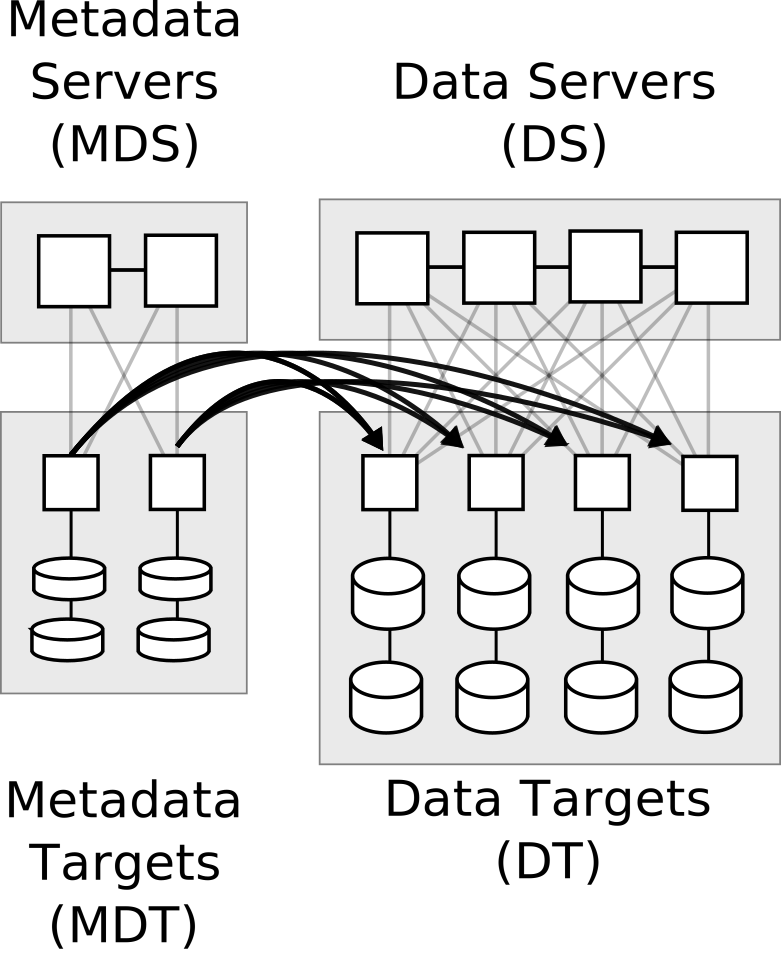
\includegraphics[width=0.33\linewidth]{use-cases/systems/storage_clean}
	\caption{A more nuanced variant of a common deployment model for storage systems. Data and metadata are handled by differently configured hardware. }
	\label{fig:System: Storage System}
\end{figure}


\paragraph{System Description:}
A system to provide (high performance) access to stored data.
Usually a large disk-based system, that exposes either a file system or an object store to read/write streams of data.
For metadata access or small random I/O (e.g. database systems) SSD-based systems are standard.
For long-term archival also automatic tape libraries are widespread.
\Cref{fig:System: Storage System} illustrates the structure of a typical online high performance distributed storage system, that also discriminates between metadata and data.

\paragraph{Risks:}
\begin{itemize}
	\item Data loss / Media Failures/Wear
	\item Performance Degradation over time / Ageing
\end{itemize}


\paragraph{Subsystems:}

\begin{itemize}
	\item I/O Servers with different configurations for metadata and data
	\item Arrays of storage media/drives
\end{itemize}


%%%%%%%%%%%%%%%%%%%%%%%%%%%%%%%%%%%%%%%%%%%%%%%%%%%%
\subsection{System: Application}
\label{System: Application}

\begin{figure}
	\centering
	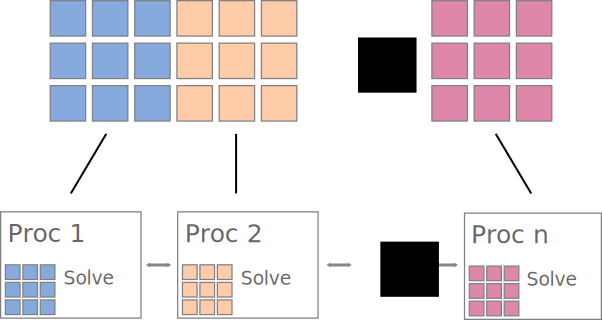
\includegraphics[width=0.5\linewidth]{use-cases/systems/application}
	\caption{A typical parallel application where work is distributed across a number of processes that collectively solve a bigger problem.}
	\label{fig:System: Application}
\end{figure}

\paragraph{System Description:}
A parallel application that utilises an HPC system to collaboratively solve a large task (for example as listed in \Cref{sec:use cases/climate and weather}).
Many applications use MPI to coordinate and exchange data across compute nodes.
\Cref{fig:System: Application} illustrates how the work represented by the colourful boxes is divided and distributed to be handled by multiple processes.

\paragraph{Risks:}
\begin{itemize}
	\item Slow to adopt changes
	%\item Maybe tightly coupled with post/pre-processing tools, CDOs
\end{itemize}


\paragraph{Subsystems:}
Applications commonly use

\begin{itemize}
	\item Library (Data Description): HDF5/NetCDF, ...  (see \Cref{System: Library})
	\item MPI: Concurrency Control and Communication %(see \Cref{System: MPI})
	%\item (Tooling): Tools either standardized or specific used for pre/post processing.
	%\item In the Future: an earth system middleware (see \Cref{System: ESDM})
\end{itemize}

%%%%%%%%%%%%%%%%%%%%%%%%%%%%%%%%%%%%%%%%%%%%%%%%%%%%
\subsection{System: Software Library (Data Description)}
\label{System: Library}


\paragraph{System Description:}
Climate/NWP codes commonly use libraries to produce portable data formats and also to some extent achieve optimised I/O performance.
Examples are HDF5, NetCDF, Adios, CDI-PIO, XIOS.


\paragraph{Risks:}
\begin{itemize}
	\item APIs may change as the library evolves, requiring Applications and an ESDM to adapt
	\item Abstractions made by the library may be inadequate in the future
\end{itemize}


\paragraph{Subsystems:}
We ignore/assume no subsystems for the software libraries for these considerations.
But it is common for a software library to depend on other specialised libraries.




%%%%%%%%%%%%%%%%%%%%%%%%%%%%%%%%%%%%%%%%%%%%%%%%%%%%
\subsection{System: ESDM}
\label{System: ESDM}

\begin{figure}
	\centering
	\includegraphics[width=0.75\columnwidth]{3rd/workflow.pdf}
	\caption{Integration and responsible of a ESDM in a climate/weather workflow.}
	\label{fig:system esdm}
\end{figure}


\paragraph{System Description:}
The earth system middleware.
The middleware sits in between the applications and plugins to interact with various data backends.
The middleware decides on the storage backend and exposes characterisations of the data centres as well as assumed data access patterns to be used by backend plugins to realise a fitting segmentation and distribution of domains in the application to storage objects and fragments.
The ESDM manages data in virtual containers and provides a data model (see \Cref{fig:System: Application} and \Cref{fig:system esdm}).
In principle, the ESDM in the use cases could be any high-level middleware.


\paragraph{Subsystems:}
We ignore/assume no subsystems except ESDM backends for the use case discussion.







%%%%%%%%%%%%%%%%%%%%%%%%%%%%%%%%%%%%%%%%%%%%%%%%%%%%
\subsection{System: Job Scheduler}
\label{System: Job Scheduler}

\paragraph{System Description:}
Users submit jobs that run an application to job schedulers.
The job scheduler will assign resources to a job and start the job.
The ESDM and the job scheduler are assumed to cooperate (see use case in \Cref{uc: simulation}.

\paragraph{Risks:}
\begin{itemize}
	\item No notable risks at this point.
\end{itemize}


\paragraph{Subsystems:}
We ignore/assume no subsystems for job schedulers.





%%%%%%%%%%%%%%%%%%%%%%%%%%%%%%%%%%%%%%%%%%%%%%%%%%
\section{Use Cases}
\label{sec:use cases/use cases}

This section covers the actual use cases as an earth system middleware addresses them.
Sub use cases are formulated to prevent use cases to become overwhelmingly complicated.
For example, it is assumed if not otherwise mentioned that the writes/reads handed to a middleware are handled as outlined in \Cref{uc: independent write} and \Cref{uc: independent read} respectively.
The particular examples for independent reads and writes are ignorant of concrete backend.
Similarly, the use case describing how simulations are handled are kept generic, so that a particular use-case for a POSIX can be swapped with a use-case that describes the handling, e.g., Lustre.
\Cref{uc: simulation} and following address current and anticipated (future) workflows used by weather and climate researchers.

Each use case features a description, involved actors, pre- and post conditions, a flow of events and exceptions.
Application use cases, in addition, have a priority rating and a description of the domain decomposition on the compute nodes and on storage.
The following list describes the content of each field in detail.


\paragraph{Use-Case Description:} A short description of the use case.

\paragraph{Priority:} A rating on the importance of this use case and a short explanation of why.

\paragraph{Actors/Systems:} The involved actors and systems (see\Cref{sec:use cases/actors} and \Cref{sec:use cases/systems}).

\paragraph{Data/Domain Description and Decomposition:} A logical description of the domain and physical domain decomposition across nodes and on the storage system.

\paragraph{Pre-Conditions:} Conditions that have to hold before the use case starts.

\paragraph{Post-Conditions:} Conditions that have to hold after the use case finished.

\paragraph{Related Use-Cases:} A list of other use cases that are related or are used by the use case.

\paragraph{Flow of Events:} A list of actions and events that are triggered as the use case is handled.

\paragraph{Exceptions:} A list of exceptions and failures that may occur and how they are handled.



%%%%%%%%%%%%%%%%%%%%%%%%%%%%%%%%%%%%%%%%%%%%%%%%
\subsection{UC: Independent Write}
\label{uc: independent write}

\paragraph{Use-Case Description:}
A process (e.g., a scientific application or a library) intends to write data using the ESDM interfaces.
The ESDM will determine a mapping and invoke a backend to write data to actual storage targets.
In addition, metadata information for later usage is written or updated.
% (also see \Cref{subsec: technical metadata}).
\Cref{fig:sequence independent write} illustrates the sequence of events in more detail.


\begin{figure}
	\centering
	\includegraphics[width=0.7\linewidth]{use-cases/uml/write/sequence.eps}
	\caption{Sequence diagram for handling independent writes. A process issues a write call to the ESDM. The middleware will create a new container if no container already exists. The ESDM collects information about the storage system and determines a domain mapping. The backends responsible for handling a certain storage system are invoked. Multiple different backends may be involved, but each backend is in charge of draining the fragment to a device. Related metadata is updated.}
	\label{fig:sequence independent write}
\end{figure}



\paragraph{Pre-Conditions:}

\begin{itemize}
	\item Parallel application with potentially multiple processes has been started
	\item ESDM has been loaded with a definition of a virtual container used for output
	\item Process: Tries to write data from a single variable to an ESDM virtual container
\end{itemize}

\paragraph{Post-Conditions:}
  \begin{itemize}
  \item Data of the variable has been transferred from process memory to some storage devices
  \item Application can reuse the memory that has been written out
  \end{itemize}

\paragraph{Flow of Events:}
\begin{enumerate}
	\item Process: announces to write a subset of data from a specific domain
	\item ESDM: identifies storage devices to store the data based on system conditions and data properties
	\item ESDM: maps domains to storage backends that will be responsible for the data.
	\item ESDM: initiates write of data by invoking backends.
	\item Storage backends: drain data onto the storage.
	\item ESDM: updates metadata.
\end{enumerate}

There are many variants of this use case depending on the conditions.






\subsection{UC: Independent Read}
\label{uc: independent read}

\paragraph{Use-Case Description:}
A process (e.g., a scientific application or a library) intends to read data using the ESDM interfaces.
The ESDM has to look up the metadata and discover available fragments. A domain filling set of fragments has to be found, and a storage backend is tasked with reading and reconstructing the requested data from the actual storage targets.
\Cref{fig:sequence independent read} illustrates the sequence of events in more detail.


\begin{figure}
	\centering
	\includegraphics[width=0.75\linewidth]{use-cases/uml/read/sequence.eps}
	\caption{Sequence diagram for handling independent reads. A process issues a read request to the ESDM. The middleware has to lookup related metadata to determine fragments required to reconstruct a domain. An ESDM storage backend will interface with the actual storage systems and fills the request buffer with the reconstructed domain.}
	\label{fig:sequence independent read}
\end{figure}



\paragraph{Pre-Conditions:}

\begin{itemize}
	\item Parallel application with potentially multiple processes has been started
	\item ESDM has been loaded with a definition of a virtual container that contains at least a single variable
	\item Process: tries to read a single variable from an ESDM virtual container
\end{itemize}

\paragraph{Post-Conditions:}
\begin{itemize}
	\item Data of the variable has been retrieved and is now available in the application as part of their domain view.
	\item The data may be cached (e.g., by the ESDM, the OS/Node or the storage system)
\end{itemize}

\paragraph{Flow of Events:}
\begin{enumerate}
	\item Process: announces to read a subset of data from a variable domain
	\item ESDM: identifies storage backends responsible for the data, i.e., map domains to storage backends.
	\item ESDM: initiates read of data on storage.
	\item Storage: provides data
\end{enumerate}






%%%%%%%%%%%%%%%%%%%%%%%%%%%%%%%%%%%%%%%%%%%%%%%%
\subsection{UC: Simulation}
\label{uc: simulation}

Simulations are the leading data producers on weather and climate-related HPC systems.
Many reading and writing clients are using the persistent storage systems (currently mostly PFS) to periodically write snapshots that can be used to continue a simulation in case of failure, but more importantly, that is used to analyse the results of simulation runs.

\paragraph{Use-Case Description:}
A user requests a job to be spawned on multiple nodes to perform a simulation of the earth system.
The simulation periodically writes out data for multiple variables. Thus the use cases assume a bursty behaviour.
The different variables are written at different frequencies.
For precise handling of the different phases refer to the section on the flow of events and \Cref{fig:sequence simulation}.
%\Cref{fig:physical simulation} illustrates the relationships of the different components from an organisational point of view.



\paragraph{Priority:}
High; The standard use-case for simulation-driven science in most data centres.

\paragraph{Actors:}
\begin{itemize}
	\item Scientist (initiating the job submission)
	\item Application (a coordinated parallel application, that collaborates collectively on something.)
	\item Process (N processes realise the application. Processes are assumed to perform work independently.
	\item ESDM
	\item Storage devices (could be anything to store, this is a generic use case)
	%\item Supercomputer (physical hardware, offers resources to be used)
	\item Workload manager (responsible for distributing jobs across the cluster hardware)
\end{itemize}


\paragraph{Data/Domain Description and Decomposition:}
A variety of different approaches to structure the logical domains of a model are possible depending on the model implementations.
This use case uses a layered two-dimensional grid in illustrations, but other structures are also possible.
\Cref{fig:domain simulation} provides a general view of the relation of processes and the grid.

Commonly, a model consists of multiple variables, and each variable may vary for a given coordinate over time.
Variables may be written at different frequencies and variables may differ in resolution.
Some simulations use multiple grids, e.g., a region may have a higher resolution than the remaining:

\begin{itemize}
	\item A 2D Grid
	\item Multiple variables
	\item Time series: per timestep, a subset of variables is stored each into a single NetCDF file
	\item Potentially multiple domains with different resolutions
	% Containers?
\end{itemize}


For simulations concerning the middleware we mainly care about how the data is distributed on the nodes, and how it later gets laid out on the storage system:

\begin{itemize}
	\item \emph{Node view:} a subset of the data domain is stored in the main memory of each node.
	%Typically, two copies are necessary: data of the previous time step is used to compute the next time step.
	\item \emph{Storage view:} somehow the data of the variables' domain is serialised into ESD variables and fragments
\end{itemize}

\begin{figure}
	\centering
	\includegraphics[width=0.5\linewidth]{use-cases/uml/simulation/domain}
	\caption{Example domain decomposition of a logical grid and how the data maybe eventually distributed across multiple processes.}
	\label{fig:domain simulation}
\end{figure}



\paragraph{Pre-Conditions:}

\begin{itemize}
	\item Input data is ready.
	\item The job is about to start by the resource manager.
	\item The user application has credentials to read the input data.
	\item Storage system has adequate health.
\end{itemize}


\paragraph{Post-Conditions:}
\begin{itemize}
	\item Written data has to be in a consistent state; ready to be read by subsequent applications.
\end{itemize}


\paragraph{Related Use-Cases:}
\begin{itemize}
	\item Uses: Independent Read (\Cref{uc: independent read})
	\item Uses: Independent Write (\Cref{uc: independent write})
\end{itemize}

%\todo{This use case most certainly splits into countless variations. Decide on a sensible subset. e.g., 1) regular grid 2) Icosahedral}


\paragraph{Flow of Events:}
\begin{enumerate}
	\item Scientist: submits a job to run an application with two defined virtual containers, one for IN and one for OUT.
	\item Workload manager: eventually allocates resources to start the job.
	  \begin{itemize}
	  \item Workload Manager: Using the information about the virtual container trigger actions, e.g., pre-staging of input data into local storage hardware or reserving bandwidth and storage space on output devices with limited capacity such as NVRAM.
	  \end{itemize}
	\item Application opens the IN container (read-only) in a collective mode.
	\item ESDM: optimises the container for read mode (optionally done during staging mode).
	\item Application opens the OUT container (write-only) in collective mode, allocate known space if necessary.
	\item ESDM: prepares the container for write mode.
	\item Application: announces to read initial simulation data.
	\item See UC: Read, it might be collective (better) or independent.
	\item Application: runs the time series of computation:
	\begin{enumerate}
		\item Process: Read auxiliary data (if necessary), see UC: Read
		\item ESDM: identifies storage devices
		\item Process: Computes (and communicates)
		\item Process: Writes a subset of variables, see UC: Write
	\end{enumerate}
	\item Application: closes the container.
	\item Application: finishes computation and terminates.
	\item Workload Manager: free the resources, manage possible stage occupied local storage resources.
\end{enumerate}


\paragraph{Exceptions:}
\begin{enumerate}
	%\item Everything works as expected the application completes N timesteps and writes M snapshots.
	\item Applications crashes between two-time steps or before regular termination.
	\item Consistency of virtual container is faulty.
	\item Network problems (Link Failure, Switch Failure) lead to premature termination of a job. ESDM has to clean up references to an incomplete container.
	\item A failure occurs when the last snapshot does not complete. As a result of the index for the last snapshot maybe broken. The ESDM has cleaned up unreferenced fragments.
\end{enumerate}


\begin{figure}
	\centering
	\includegraphics[width=\linewidth]{use-cases/uml/simulation/sequence.eps}
	\caption{Sequence diagram for the simulation use case. A user submits a job with IN and OUT destinations specified. A job manager will spawn the actual job by allocating nodes and order to start the application code on each node. Usually, simulations need to read in a set of initial conditions. It will then iteratively compute one time step after another, while occasionally (usually at fixed frequencies which may vary per variable) writing snapshot data to be used during analysis or to restart an interrupted simulation.}
	\label{fig:sequence simulation}
\end{figure}


%\begin{figure}
% 	\centering
% 	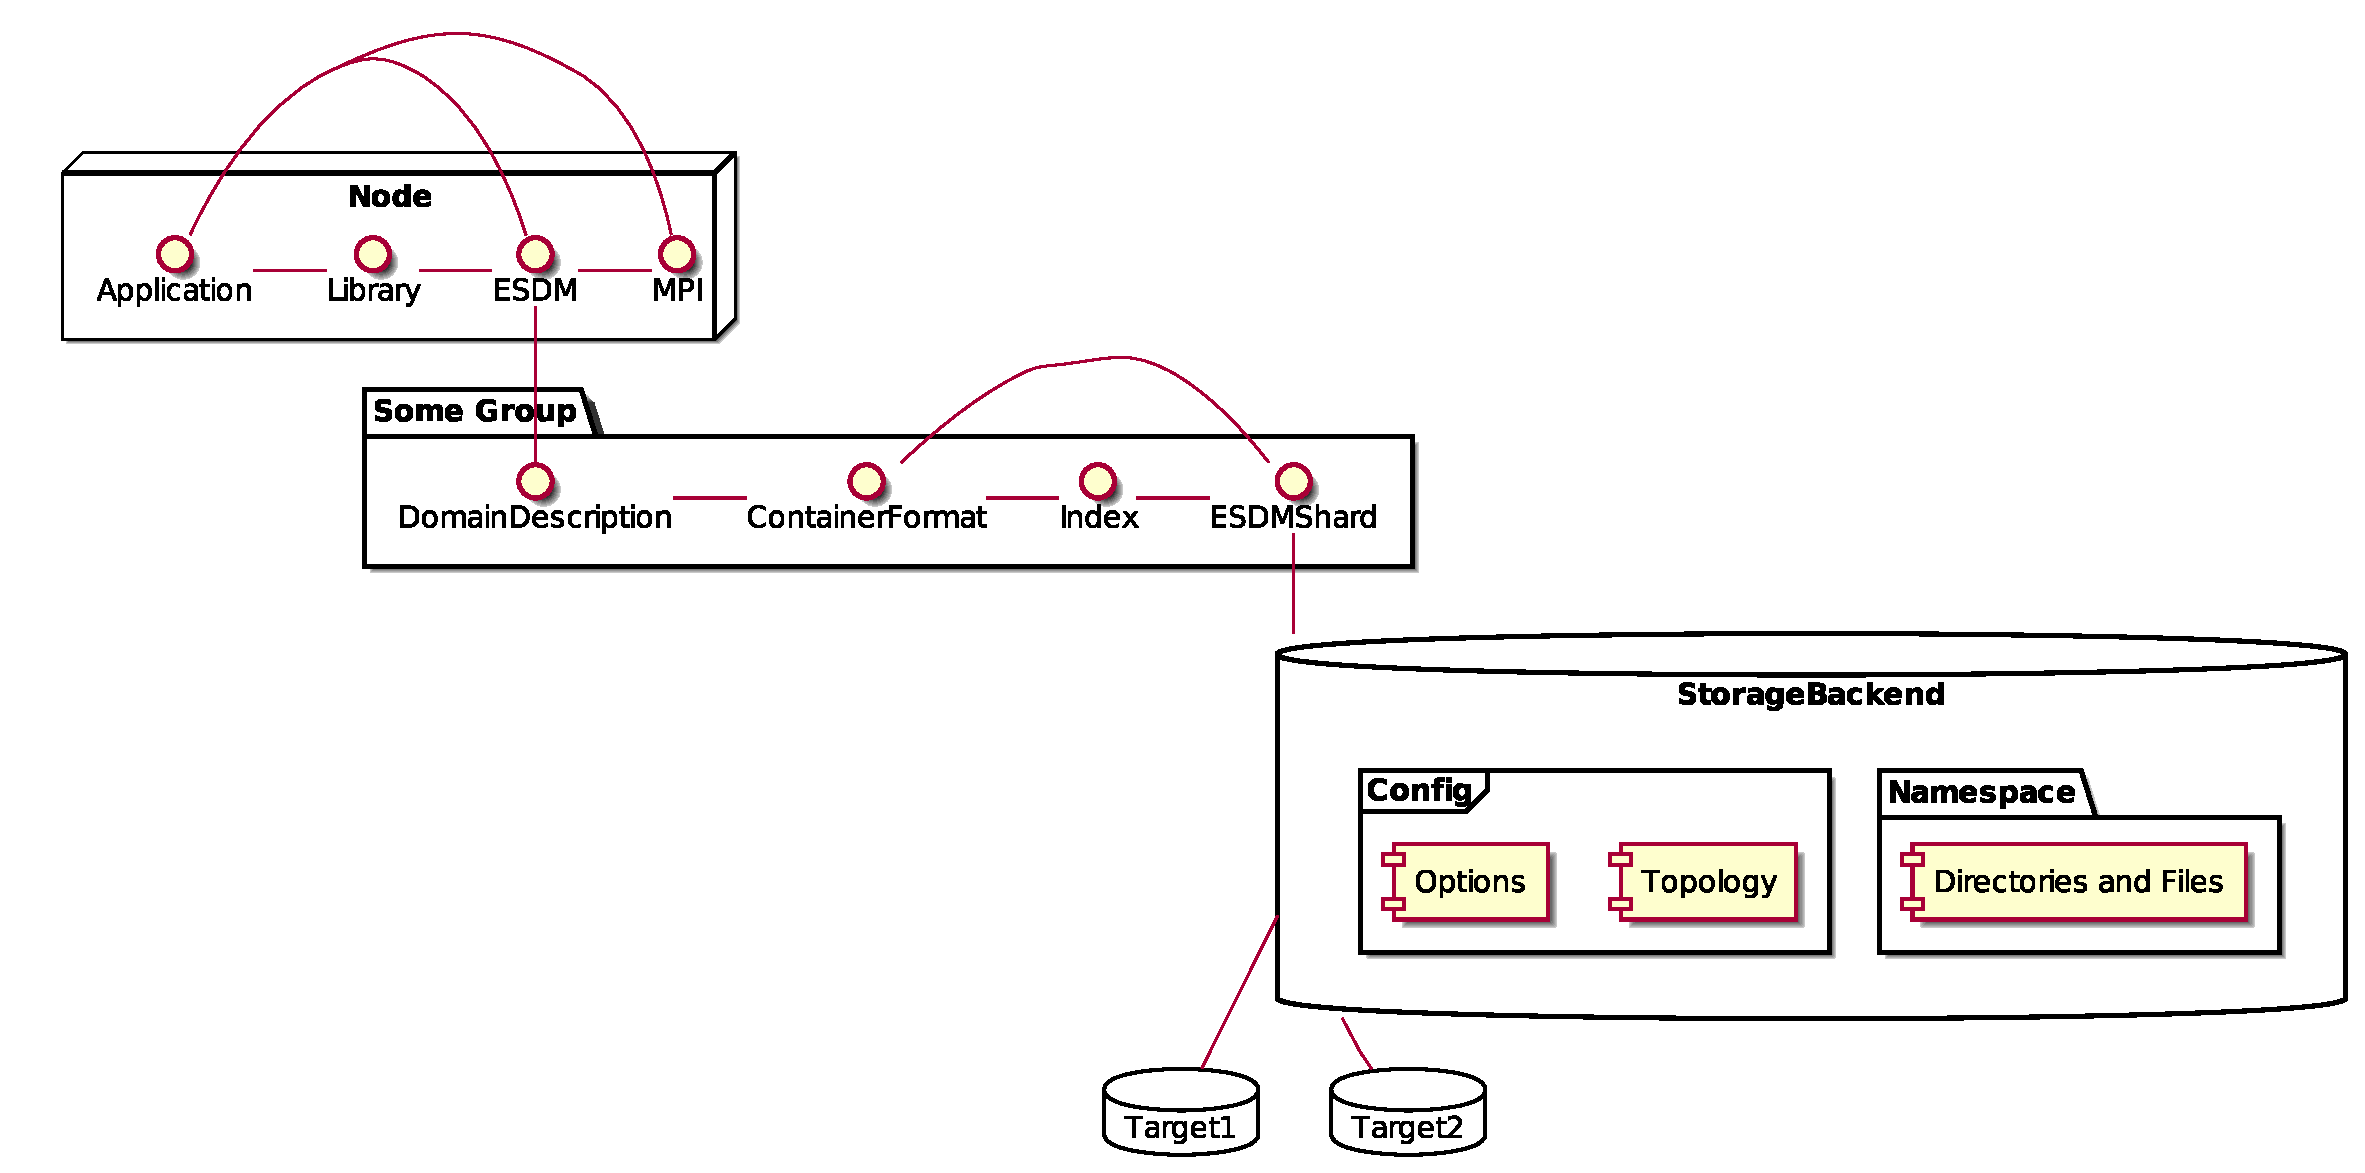
\includegraphics[width=\linewidth]{use-cases/uml/simulation/participants.eps}
% 	\caption{View of participants and their relations. An application is likely to interface with the ESDM only indirectly through a library. Applications as well as the ESDM coordinate using MPI. Each node running the simulation is has loaded the application code, libraries, the ESDM and MPI as well as memory that is managed by each of these. Within the ESDM different submodules are active that handles the domain description, interpret the container format and ESDM fragments. For the storage backend, an administrator has to provide configuration information such as the topology and the namespace organisation.}
% 	\label{fig:physical simulation}
% \end{figure}







%%%%%%%%%%%%%%%%%%%%%
\subsection{UC: Pre/Post Processing on a existing Data}
\label{uc: pre + post processing}

Before a simulation can run, input data from satellites, weather stations and other sources has to be converted into a representation that matches the grid of the simulation.
Similarly, simulations output a lot of raw data to be flexible to perform at simulation-time unexpected analysis.
Pre- and post-processing jobs are therefore an integral part of the workload mix at supercomputing sites but also on smaller local installations.


\paragraph{Use-Case Description:}
A user submits a pre/post processing job to the workload manager requiring to read data sets from one or more input sources.
Ideally, the task is described using a standard tool or a framework for data transformations (e.g. CDO).
There are countless possibilities for the type of calculations performed and for the regions that need to be accessed in the logical domain (see \Cref{fig:domain pre + post processing})
Many analysis workloads access time series data, thus require to access similarly-structured files with the same pattern.
\Cref{fig:sequence pre + post processing} illustrates the sequence of events in more detail.

\paragraph{Priority:} High. Researchers routinely have to perform pre/post-processing

\paragraph{Actors:}
\begin{itemize}
	\item Scientist
	\item Pre/Post Processing Application (e.g. CDO)
	\item Supercomputer
	\item ESDM
\end{itemize}


\paragraph{Data/Domain Description and Decomposition:}
In alignment with the other use cases, a Cartesian grid is assumed, but many other grids are in principle handled similarly.
\Cref{fig:domain pre + post processing}
%\todo{text in the figure: stripe size 5- may bestride you mean?  Some systems call it stride some call it stripe. On instance with lustre which uses strips in the same context as in the picture..  https://www.nics.tennessee.edu/computing-resources/file-systems/lustre-striping-guide }
 illustrates the logical decomposition, an example serialisation and the distribution across a storage system.
The producing application decided for which access pattern the serialisation is favourable. In many situations, the provided serialisation is suboptimal for the transformation.


\begin{figure}
	\centering
	\includegraphics[width=\linewidth]{use-cases/uml/prepost-processing/domain}
	\caption{The logical domain view, a serialisation and how it is striped across a storage system. The grey grids below illustrate possible access patterns, but the layout on storage is not optimal for any of the shown access patterns. }
	\label{fig:domain pre + post processing}
\end{figure}


\paragraph{Pre-Conditions:}
\begin{itemize}
	\item Data set is available via ESDM (because of producer termination or epoch)
	\item The data set may be available, but may have suboptimal fragmentation.
	\item A common description/framework for post-processing is used (e.g. CDO)
\end{itemize}

\paragraph{Post-Conditions:}
\begin{itemize}
	\item The pre/post processing region of interest result is accessible by the user.
	\item The data set container is improved by additional indexes or additional fragments for faster access next time.
\end{itemize}

\paragraph{Related Use-Cases:}
\begin{itemize}
	\item Uses: Independent Read (\Cref{uc: independent read})
	\item Uses: Independent Write (\Cref{uc: independent write})
\end{itemize}


\paragraph{Flow of Events:}
\begin{enumerate}
	\item Scientist: submits a post-processing job, multiple virtual containers for INPUT and OUTPUT may be specified.
	\item Workload Manager: eventually allocates resources and starts the job.
	\item Pre/Post processing may open multiple files one after another (e.g. time series)
	\begin{enumerate}
	\item Process: opens the INPUT  (see UC: Read \Cref{uc: independent read})
	\item Process: performs transformation or analysis (e.g. compute average)
	\end{enumerate}
	\item Process: Writes a transformed data set (see UC: Write \Cref{uc: independent write})
	\item Process: Possibly creates plot or film of analysis.
\end{enumerate}


\begin{figure}
	\centering
	\includegraphics[width=\linewidth]{use-cases/uml/prepost-processing/sequence}
	\caption{Sequence diagram for the flow of events for a stand-alone pre/post processing task. Depending on the analysis task, no output may occur until all data from a time series was gathered.}
	\label{fig:sequence pre + post processing}
\end{figure}



\paragraph{Exceptions:}
\begin{enumerate}
	\item  Requiring to ensure clean up of unreferenced/inconsistent data is inherited from Read/Write use cases (see \Cref{uc: independent read} and \Cref{uc: independent write})
\end{enumerate}



%
%\todo{
%	Domain, subdomain, coordinates
%
%	Layout component index:
%	- Coordinates are in fragment Z; does NOT tell where in the fragment
%	- Optimize the number of fragments to query
%	- Performance predictor für jedes PFS ?	\item
%
%	PFS index:
%	- File: sequence(metadata + pointer to last metadata + data ), index (with pointer to all metadata blocks)
%	Mapping from multidimensional coordinates to byte offset and array
%	Many different representations are possible
%
%	Potentially more than one fragment into one file (optimize metadata for millions of procs).
%
%}
%



%%%%%%%%%%%%%%%%%%%%%%%%%%%%%%%%%%%%%%%%%%%%%%%
\subsection{UC: Concurrent Simulation and Post-Processing for Pipelines/Workflows}
\label{uc: pipeline}

For weather prediction, it is common to have post-processing pipelines responsible for the generation of value-added services.
In expectancy of a formal definition of workflows and increased use of containerisation this use case describes how an ESDM would need to realise automatic post-processing as soon as data becomes available.


\paragraph{Use-Case Description:}
A processing pipeline is set up that regularly receives new input data, for example, measurement data from a satellite system.
Periodically, the most recent satellite data is fed to simulation as input (see \Cref{uc: simulation}).
As simulations write snapshots, value-added products are generated in post-processing steps.
For example in an NWP setting warnings or a weather forecast (compare \Cref{sec:use cases/climate and weather}).
\Cref{fig:sequence pipeline} illustrates the sequence of events in more detail.




\paragraph{Priority:}
Low - Not in scope of the project to integrate with in-situ post-processing tools.
Also, other systems such as the workload manager need to be adapted to support this.


\paragraph{Actors:}
\begin{itemize}
	\item Scientist
	\item Application
	\item Supercomputer
	\item ESDM
	\item Pre/Post Processing Framework
\end{itemize}


\paragraph{Data/Domain Description and Decomposition:}
The input data may be in various formats with a domain layout that is not optimal for the simulation.
For simplicity, conversion steps are omitted in the description, but if necessary a transformation would correspond to UC: Pre/Post Processing (see \Cref{uc: pre + post processing}).
\Cref{fig:domain workflow} illustrates an observation system that provides data in portable container format (could also be an ESDM container).
The observation data is then used as initial conditions for a simulation, the domain decomposition and resulting output matches the description in UC: Simulation (see \Cref{uc: simulation}).
Finally, the output data is post-processed for which the domain description, again, corresponds to UC: Pre/Post Processing (see \Cref{uc: pre + post processing}).


\begin{figure}
	\centering
	\includegraphics[width=\linewidth]{use-cases/uml/pipeline/domain}
	\caption{Illustration of the domain and a possible pipeline. New observational data is constantly added, and then used in simulations. The simulation output is then used by post processing tasks to compile specific forecasts and warnings.}
	\label{fig:domain workflow}
\end{figure}




\paragraph{Pre-Conditions:}
\begin{itemize}
	\item Sufficient resources to start simulations and post-processing workloads available.
	\item A pipeline is provided in a machine-readable format.
	\item Simulation preconditions as described in UC: Simulation applies (\Cref{uc: simulation})
	\begin{itemize}
		\item Input data is ready.
		\item The job is about to start by the resource manager.
		\item The user application has credentials to read the input data.
		\item Storage system has adequate health.
	\end{itemize}

\end{itemize}


\paragraph{Post-Conditions:}
\begin{itemize}
	\item Post processing can compute results as soon as an epoch completes.
	\item Combined task is hopefully faster than traditional approaches (generate, write, [read, transform, write], read, post-process, write result)
\end{itemize}


\paragraph{Related Use-Cases:}
\begin{itemize}
	\item Uses: Independent Read (\Cref{uc: independent read})
	\item Uses: Independent Write (\Cref{uc: independent write})
	\item Adapts: Simulation (\Cref{uc: simulation})
	\item Adapts: Pre/Post processing on an existing Data (\Cref{uc: pre + post processing})
\end{itemize}


\paragraph{Flow of Events:}
\begin{enumerate}
	\item Observation System: Observations are constantly stored and timestamped.
	\item ESDM: handles storage on the storage system and potentially transforms data as needed by pipeline/workflow.
	\item Workload Manager: periodically allocate resources to spawn new jobs with most recent data
	\begin{enumerate}
		\item Application: A simulation is started as outlined in UC: Simulation (\Cref{uc: simulation})
		\item Application: opens the INPUT (see UC: Read \Cref{uc: independent read})
		\item ESDM: Serves the input and transform data.
		\item Application: Loop
			\begin{enumerate}
				\item Application: writes subset of variables
				\item ESDM: makes data available to post processing immediately (e.g., inform workload manager to schedule post processing job)
				\item ESDM: writes snapshot asynchronously
			\end{enumerate}
	\end{enumerate}
	\item Repeat.
\end{enumerate}

\begin{figure}
	\centering
	\includegraphics[width=\linewidth]{use-cases/uml/pipeline/sequence.eps}
	\caption{Sequence Diagram for Concurrent Simulation and Post processing for Pipelines/Workflows}
	\label{fig:sequence pipeline}
\end{figure}




\paragraph{Exceptions:}
Multiple failure modes are possible, but they are all inherited by the used use cases only may require cleaning up inconsistent/incomplete fragments and containers:

\begin{enumerate}
	\item Simulations can fail (see UC: Simulation \Cref{uc: simulation})
	\item Pre/Post Processing of existing data may also fail (see \Cref{uc: pre + post processing})
\end{enumerate}


%%%%%%%%%%%%%%%%%%%%%%%%%%%%%%%%%%%%%%%%%%%%%%%
\subsection{UC: Simulation + In situ post processing}
\label{uc: simulation + in-situ + post processing}

A common problem with post-processing applications is that data is first written to storage, just to be read again from another consumer for post-processing.
This process unnecessarily stresses the storage system, because if it is known in advance that an average for an area needs to be calculated, then the generating application can notify or perform the post-processing on the node where the data is already present.


\paragraph{Use-Case Description:}
A job is spawned on multiple nodes which collectively run a simulation of the earth system (see \Cref{uc: simulation}).
The job contains information about necessary post-processing steps.
Alternatively, the job may be part of the workflow, and the post-processing steps are derived from the workflow.
As the simulation proceeds, several post-processing calculations are performed directly on the nodes that already hold the generated data.
\Cref{fig:sequence in-situ} illustrates the sequence of events in more detail.

\paragraph{Priority:} Low - Not in scope of the project to integrate with in-situ post-processing frameworks.


\paragraph{Actors:}
\begin{itemize}
	\item Scientist
	\item Application
	\item Supercomputer
	\item ESDM
	\item Pre/Post Processing Framework
\end{itemize}


\paragraph{Data/Domain Description and Decomposition:}
The logical model domain corresponds to the domain description and decomposition in the UC: Simulation (see \Cref{uc: simulation}).
Candidates for in-situ post-processing can be derived from UC: Pre/Post-processing on an existing Data (\Cref{uc: pre + post processing}).
\Cref{fig:domain simulation+insitu+postproc} illustrates how the domains are decomposed and which computational loads are performed by a specific process (only simulation or simulation with post-processing).

%\begin{itemize}
%	\item Node: Variable, a tuning parameter usually maximise ram usage for model data.. commonly two copies for the current and previous time step.
%	\item Storage: PFS default configuration?
%\end{itemize}


\begin{figure}
	\centering
	\includegraphics[width=0.5\linewidth]{use-cases/uml/simulation+insitu+postproc/domain}
	\caption{The logical domain is decomposed and distributed across multiple processes. The darker cells denote a region that requires post-processing. The processes assigned to handle these regions are also tasked to compute a post-processing result directly. This way it is possible to avoid unnecessary reading from the storage system for known post-processing tasks.}
	\label{fig:domain simulation+insitu+postproc}
\end{figure}




\paragraph{Pre-Conditions:}
\begin{itemize}
	\item The post-processing tasks are indicated in the job script or workflow.
	\item This use case inherits the preconditions of UC: Simulation (\Cref{uc: simulation})
\end{itemize}


\paragraph{Post-Conditions:}
\begin{itemize}
	\item All simulation output data is now in a consistent state and ready to be read by subsequent applications.
	\item Post-processing tasks on a subset of the domain are completed without requiring first to write and then again.
	\item The post-processing results are written in a consistent state.
	% durable -- persisted onto non-volatile storage.
	%\item Indexes are healthy to receive data.
\end{itemize}



\paragraph{Related Use-Cases:}
\begin{itemize}
	\item Uses: Independent Read (\Cref{uc: independent read})
	\item Uses: Independent Write (\Cref{uc: independent write})
	\item Extends: Simulation (\Cref{uc: simulation})
	\item Extends: Pre/Post processing on an existing Data (\Cref{uc: pre + post processing})
\end{itemize}


\paragraph{Flow of Events:}
\begin{enumerate}
	\item Scientist: submits jobs to run an application with containers for input and output specified. In addition, a list of required post-processing is provided (provided by the job script, derived from a workflow or possibly learned automatically).
	\item Workload manager: eventually allocates resources to start a job. (ESDM can optimise before job start see \Cref{uc: simulation}).
	\item Application opens the IN container (read-only) in a collective mode.
	\item ESDM: optimises the container for read mode (optionally done during staging mode).
	\item Application opens the OUT container (write-only) in collective mode, allocate known space if necessary.
	\item ESDM: prepares the container for write mode.
	\item Application: announces to read initial simulation data.
	\item See UC: Read, it might be collective (better) or independent.
	\item Application: runs the time series of computation:
	\begin{enumerate}
		\item Process: Reads auxiliary data (if necessary), see UC: Read
		\item ESDM: identifies storage devices
		\item Process: Computes (and communicate)
		\item Process: Writes a subset of variables, see UC: Write
		\item ESDM: As data becomes available post-processing tasks are executed
		\item Post Processing Framework: (only by affected processes) performs post-processing
	\end{enumerate}
	\item Application: closes the container.
	\item Application: finishes computation and terminates.
	\item Workload Manager: free the resources, potentially unstaged occupied local storage resources.
\end{enumerate}


\begin{figure}
	\centering
	\includegraphics[width=\linewidth]{use-cases/uml/simulation+insitu+postproc/sequence.eps}
	\caption{Sequence Diagram for Simulation + In situ post processing.}
	\label{fig:sequence in-situ}
\end{figure}




\paragraph{Exceptions:}
\begin{enumerate}
	\item Simulation can fail and if snapshots are being written consistency checks need to be performed, and unnecessary fragments require clean up (see UC: Simulation \Cref{uc: simulation}).
	\item Post processing could fail
\end{enumerate}


%\paragraph{Subordinate Use-Cases:}
%\begin{itemize}
%	\item For special cases that are not adequate as a scenario. If any.
%\end{itemize}



%%%%%%%%%%%%%%%%%%%%%%%%%%%%%%%%%%%%%%%%%%%%%%%
\subsection{UC: Simulation + In situ + Interactive Visualisation}
\label{uc: simulation + in-situ + cam}


Periodically writing snapshots of the model state typically slows down the simulations considerably, because the simulation has to wait for the I/O systems to finish writing a snapshot before it can continue.
Additional resources such as I/O nodes or burst buffers can be used to flush data asynchronously from the application and, thus, prevents climate applications from waiting for I/O.
An alternative can be to inspect simulations directly by using in-situ visualisation.
\Cref{uc: simulation + big data + in-situ} describes a similar use case that applies big data analytics to detect anomalies before notifying a user for in-situ inspection.


\paragraph{Use-Case Description:}
A job is spawned on multiple nodes which collectively run a simulation of the earth system (see \Cref{uc: simulation}).
As the simulation proceeds, a user can render the current state of the simulation using a visualisation tool.
Over time, the user may choose to change the camera view, which variables are included in the visualisation.
\Cref{fig:sequence simulation + in-situ + cam} illustrates the sequence of events in more detail.

\paragraph{Priority:}
Low - Not in scope of the project to integrate with in-situ frameworks.

\paragraph{Actors:}
\begin{itemize}
	\item Scientist
	\item Application
	\item Supercomputer
	\item Visualisation	Cluster
	\item ESDM
\end{itemize}


\paragraph{Data/Domain Description and Decomposition:}
The logical model domain corresponds to the domain description and decomposition in the UC: Simulation (compare to \Cref{uc: simulation}).
In addition, the camera window requires to be rendered:
Depending on the position of the camera, different compute nodes, and visualisation nodes have to communicate (see \Cref{fig:domain simulation + in-situ + cam}).
Each visualisation node is only responsible for the defined region of the camera's view (e.g. top left quarter of the domain).


\begin{figure}
	\centering
	\includegraphics[width=0.5\linewidth]{use-cases/uml/simulation+insitu+camara/domain}
	\caption{Domain Illustration}
	\label{fig:domain simulation + in-situ + cam}
\end{figure}



\paragraph{Pre-Conditions:}
\begin{itemize}
	\item Input and output destinations are accessible to the user.
	\item An allocation to a supercomputer is granted by the resource manager.
	\item An allocation to a visualisation cluster is granted (possibly part of the same supercomputer).
\end{itemize}


\paragraph{Post-Conditions:}
From an ESDM perspective, no post-conditions have to hold because no data is written.
Alternatively, if a user decides to start storing snapshots, the post-conditions of UC: Simulation applies (see \Cref{uc: simulation}).




\paragraph{Related Use-Cases:}
\begin{itemize}
	\item Adapts: Simulation (\Cref{uc: simulation})
\end{itemize}


\paragraph{Flow of Events:}
\begin{enumerate}
	\item Scientist: submits jobs to run on an application with containers for input and output specified. In addition, a list of required post-processing is provided (provided by the job script, derived from a workflow or possibly learned automatically).
	\item Workload manager: eventually allocates resources to start a job. (ESDM can optimise before job start see \Cref{uc: simulation}).
	\item Application opens the IN container (read-only) in a collective mode.
	\item ESDM: optimises the container for read mode (optionally done during staging mode).
	\item Application opens the OUT container (write-only) in collective mode, allocate known space if necessary.
	\item ESDM: prepares the container for write mode.
	\item Application: announces to read initial simulation data.
	\item See UC: Read, it might be collective (better) or independent.
	\item Application: runs the time series of computation:
	\begin{enumerate}
		\item Process: Reads auxiliary data (if necessary), see UC: Read
		\item ESDM: identifies storage devices
		\item Process: Computes (and communicate)
		\item Process: Writes a subset of variables
		\item ESDM: receives data and data is only buffered for a limited number of timesteps
		\item ESDM: exchanges data within camera view to visualisation nodes
		\item Visualisation: Renders a frame for the current view (as a user moves camera rerenders may become necessary if not cached)
	\end{enumerate}
	\item Application: finishes computation and terminates.
	\item Workload Manager: free the resources, manage possible stage occupied local storage resources.
\end{enumerate}


\begin{figure}
	\centering
	\includegraphics[width=\linewidth]{use-cases/uml/simulation+insitu+camara/sequence.eps}
	\caption{Sequence Diagram}
	\label{fig:sequence simulation + in-situ + cam}
\end{figure}



\paragraph{Exceptions:}
\begin{enumerate}
	\item Simulation can fail and if snapshots are being written consistency checks need to be performed, and unnecessary fragments require clean up (see UC: Simulation \Cref{uc: simulation}).
	\item Visualisation cluster may fail. It could be a responsibility of the ESDM to re-spawn the visualisation In terms of data consistency the ESDM requires no actions.
\end{enumerate}





%%%%%%%%%%%%%%%%%%%%%%%%%%%%%%%%%%%%%%%%%%%%%%%
\subsection{UC: Simulation + Big Data Analysis + In situ analysis/visualisation}
\label{uc: simulation + big data + in-situ}

Inline with the previous in-situ use cases (see \Cref{uc: simulation + in-situ + post processing} and \Cref{uc: simulation + in-situ + cam}), the goal is to take the stress off the storage system, in this case by being more selective about which snapshots are permanently stored.
Big data tools in combination with machine learning techniques promise to allow computers to apply sophisticated analysis tasks on large amounts of data automatically.
Such analysis is already applied to satellite data, e.g. to track biodiversity, combating desertification or detect wildfires.
In the future, this might also be applied to faux satellite images generated from model output (or the raw data directly) to better characterise the impact on various environmental factors of climate policy actions.



\paragraph{Use-Case Description:}
A parallel job is started in which multiple nodes collectively simulate the earth system (see \Cref{uc: simulation}).
As the simulation runs, no data is written but using big data analytics anomalies of interest are detected.
A configuration defines what actions are triggered.
Additional jobs could be started, or a scientist is notified about an anomaly to perform further analysis jobs or use visualisation.
\Cref{fig:sequence simulation + big data + in-situ} provides a sequence diagram on the flow of events for this use case.

\paragraph{Priority:}
Low - Not in scope of the project to integrate with in-situ frameworks and big data cluster systems.

\paragraph{Actors:}
\begin{itemize}
	\item Scientist
	\item Application
	\item Supercomputer
	\item Big Data Analysis Cluster (this could also be the supercomputer)
	\item ESDM
	\item Pre/Post Processing Framework
\end{itemize}


\paragraph{Data/Domain Description and Decomposition:}
Multiple domain decompositions are at play in this use case.
The simulation decomposition corresponds to the description in UC: Simulation (\Cref{uc: simulation}) except that we assume no snapshots are permanently stored until a trigger condition occurs.
The big data analysis workloads do not follow a fixed structure and heavily depend on the analysis performed.
UC: Pre/Post Processing (see \Cref{uc: pre + post processing}) illustrated multiple possible access patterns which also apply here.
A more sophisticated analysis may also be responsive to the time evolution within a simulation. For example, a storm might move within the simulation, and the analysis could follow the storm generating a situation similar to UC: Simulation + Interactive in-situ visualisation (compare to {uc: simulation + in-situ + cam}) is more appropriate.


%\begin{figure}
%	\centering
%	\includegraphics[width=\linewidth]{use-cases/uml/simulation+insitu+camara/sequence.eps}
%	\caption{Sequence Diagram}
%	\label{fig:sequence simulation + big data + in-situ}
%\end{figure}


\paragraph{Pre-Conditions:}
\begin{itemize}
	\item Pre-conditions as with UC: Simulation
	\item User has nodes allocated for Big Data Analysis
	\item Available resources to add jobs as required for pre-processing
\end{itemize}

\paragraph{Post-Conditions:}
\begin{itemize}
	\item Data that users want to preserve is permanently stored
\end{itemize}




\paragraph{Flow of Events:}
\begin{enumerate}
	\item Scientist: submits jobs to run an application with containers for input and output specified. In addition, a list of required post-processing is provided (provided by the job script, derived from a workflow or possibly learned automatically).
	\item Workload manager: eventually allocates resources to start a job. (ESDM can optimise before job start see \Cref{uc: simulation}).
	\item Application opens the IN container (read-only) in a collective mode.
	\item ESDM: optimises the container for read mode (optionally done during staging mode).
	\item Application opens the OUT container (write-only) in collective mode, allocate known space if necessary.
	\item ESDM: prepares the container for write mode.
	\item Application: announces to read initial simulation data.
	\item See UC: Read, it might be collective (better) or independent.
	\item Application: runs the time series of computation:
	\begin{enumerate}
		\item Process: Read auxiliary data (if necessary), see UC: Read
		\item ESDM: identifies storage devices
		\item Process: Computes (and communicate)
		\item Process: Writes a subset of variables
		\item ESDM: receives data but no permanent data is stored yet
		\item ESDM: makes data available to big data analysis cluster (e.g. burst buffer)
		\item Big Data Cluster: performs analysis (this may take a while)
		\item ESDM: eventually analysis receives a result. If trigger condition matches:
		\begin{enumerate}
			\item ESDM: may notify the user
			\item ESDM: may start to write snapshots
			\item ESDM: may invoke callback/run script
		\end{enumerate}
	\end{enumerate}
	\item Application: closes the container.
	\item Application: finishes computation and terminates.
	\item Workload Manager: free the resources, manage evtl. stage occupied local storage resources.
\end{enumerate}



\begin{figure}
	\centering
	\includegraphics[width=\linewidth]{use-cases/uml/simulation+insitu+bigdata/sequence.eps}
	\caption{Sequence Diagram}
	\label{fig:sequence simulation + big data + in-situ}
\end{figure}



\paragraph{Related Use-Cases:}
\begin{itemize}
	\item Adapts: Simulation (\Cref{uc: simulation})
	\item Adapts: Pre/Post Processing on existing data (\Cref{uc: pre + post processing})
\end{itemize}






\paragraph{Exceptions:}
\begin{enumerate}
	\item Simulation can fail and if snapshots are being written consistency checks need to be performed, and unnecessary fragments require clean up (see UC: Simulation \Cref{uc: simulation}).
	\item Big data cluster may fail. It could be a responsibility of an ESDM to resubmit tasks for analysis.
\end{enumerate}
